\documentclass[pdftex,a4paper,12pt]{report}

\usepackage{algorithm2e}
\usepackage{amsmath}
\usepackage{hyperref}
\usepackage{color}
\usepackage{fullpage}
\usepackage{graphicx}
\renewcommand{\thesection}{\arabic{section}}

\hypersetup{
  colorlinks,
  citecolor=blue,
  linkcolor=blue,
  urlcolor=blue
}
\begin{document}
\begin{titlepage}
\begin{center}

\textsc{\LARGE IIT Kanpur}\\[1.5cm]

\textsc{\Large CS345A - AlgorithmsII}\\[0.5cm]

% Title
{ \huge \bfseries Assignment 1 \\[0.4cm] }


\begin{minipage}{0.4\textwidth}
\begin{flushleft} \large
Anjani Kumar\\
11101
\end{flushleft}
\end{minipage}
\begin{minipage}{0.4\textwidth}
\begin{flushright} \large
Sumedh Masulkar\\
11736
\end{flushright}
\end{minipage}

\vfill

% Bottom of the page
{\large January 12, 2014}

\end{center}
\end{titlepage}

\tableofcontents
\newpage
\section {Non Dominated Points}
\subsection {\textbf{$O(n logn)$} algorithm for non-dominated points in a plane.}

\paragraph{Overview of algorithm} 
Given set of points $P$ in a plane. \\
Divide Step:
\begin{enumerate}
\item
If there is only one point in a plane, the point itself is non-dominated set of points. Hence, return $P$.
\item
If there are two points, if any point has both x and y co-ordinates both greater than that of other point, then return that point, else return $P$.
\item
Else find the x-median of the points and divide the plane into left half plane and right half plane using the median. And now call the function for both the half planes.\\
\end{enumerate}
Conquer Step:\\
Goal: Given the non-dominated points of the two half planes, merge the solution of smaller parts to get the solution of the bigger plane.\\\\
Assuming we have two sets of points $P_1$ and $P_2$, where $P_1$ is the set of non-dominated points of the left plane, and $P_2$ is the set of non-dominated points of the right plane respectively. \\\\
The x-coordinate of all the points in right plane are obviously greater than x-coordinate of all the points in the left plane. Thus, we only need to eliminate points from $P_1$ that are dominated by points in $P_2$.\\
Since x-coordinate of points in $P_2$ is always greater, we only need to look for the y-coordinates.\\
Let y be the point in $P_2$ with maximum y-coordinate. Then the dominated points in $P_1$ are all the points whose y-coordinates are less than y-coordinate of y.\\
Thus the solution of the plane will be \{ $P_1$ - \{points in $P_1$ with y-coordinate $<$ y \} \} $\cup P_2$. \\

\pagebreak

\paragraph{Pseudo-Code.} \mbox{} \\\\
\begin{algorithm}

NonDominatedPts(set of points P)\{\\
\makebox[40pt]{}\textcolor{blue}{//Returns set of non dominated points from $P$.}

      \uIf{$\mid$P$\mid$==1} {return P\;}
      \uElseIf{$\mid$P$\mid$==2}{
	    let $p_1$ and $p_2$ be the two points in P\;
	    \uIf {$x_1 > x_2$ and $y_1 > y_2$}{ return \{$p_1$\};	\qquad	\textcolor{blue}{//$p_1$=($x_1$,$y_1$), and $p_2$=($x_2$,$y_2$)}}
	    \uElseIf{$x_1 < x_2$ and $y_1 < y_2$} {return \{$p_2$\}\;}   
	    \uElse{return P;}
      }
      \uElse{
	    p* $\gets$ x-median(P);			\makebox[200pt]{}\textcolor{red}{//$c_1$n}\\
	    (L,R) $\gets$ split(P, p*);		\makebox[190pt]{}\textcolor{red}{//$c_2$n}\\
	    $P_1$ $\gets$ NonDominatedPts(L);		\makebox[130pt]{}\textcolor{red}{//T(n/2)}\\
	    $P_2$ $\gets$ NonDominatedPts(R);		\makebox[130pt]{}\textcolor{red}{//T(n/2)}\\
	    $P_1$ $\gets$ $P_1$ sorted along y-axis;	\makebox[140pt]{}\textcolor{red}{//$c_3$n}\\
	    y $\gets$ max y-coordinate in points of $P_2$;	\makebox[80pt]{}\textcolor{red}{//$c_4$n}\\
	    $P_1$ $\gets$ $P_1$ - \{all points in $P_1$ whose y-coordinate $\leq$ y\};\makebox[30pt]{}\textcolor{red}{//$c_5$n}\\
	    return ($P_1\cup P_2$);\\
      }
\}
\caption{\textbf{$O(n logn)$} algorithm to find Non Dominated Points}
\label{alg}
\end{algorithm}

\paragraph{Time Complexity:} \textbf{$O(n)$} + 2T(n/2) = \textbf{$O(n logn)$}.
\newpage

\paragraph{Proof of Correctness:} \makebox[2pt]{}\\
\begin{figure}[ht!]
\centering
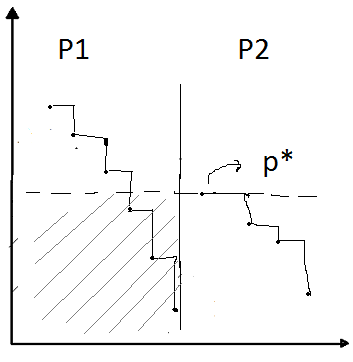
\includegraphics[width=60mm]{p1.png}
\caption{Figure for non-dominated pts}
\label{fig}
\end{figure}

Proof by induction on size of set P.
\begin{itemize}
 \item If($\mid$P$\mid$=1), the point is non-dominated, hence the set P should be returned.
 \item If($\mid$P$\mid$=2), Remove dominanted point if exists, and return P.
 \item \textbf{Induction Hypothesis: } The solution of both half planes, $P_1$ and $P_2$ are known, $i.e.$ now $P_1$ and $P_2$ consist only of 
 non-dominated points among themselves. And we need to merge their solution to get solution of $P$.\\
 As shown in figure, the points in $P_2$ cannot be dominated by any point in $P_2$(according to induction hypothesis) or $P_1$(since x-coordinate of any point
 in $P_2$ is greater than x-coordinate of any point in $P_1$).\\
 See figure(\ref{fig}).\\
 If p* is the point with maximum y-coordinate in $P_2$, no point in $P_1$ which has y-coordinate greater than that of p* can be dominated by any point
 in $P_1$(by induction hypothesis) or $P_2$(since y-coordinate is greater than that of p*).\\
 Thus, the group of points in $P_1$ that have y-coordinate less than that of p* are dominated(x-coordinate is also less).\\
 Hence, we need to remove this group of points from $P_1$ and remaining $P_1 \cup P_2$ will be the answer.\\
 Thus, the algorithm is correct.
\end{itemize}

\newpage

\subsection {\textbf{$O(n logh)$} algorithm for non-dominated points in a plane}
\paragraph{Idea} \makebox[2pt]{}\\

The solution to this problem is similar to that of algorithm \ref{alg}, with a slight modification.
Here, we are removing the dominated group of points from $P_1$ (see fig. \ref{fig}), before we find non-dominated points of $P_1$,
hence reducing the number of points NonDominatedPts($P_1$) returns($h_1$), in the following analysis. 

\paragraph{Time Complexity Analysis:}\makebox[2pt]{}\\\\
$T(n,h)$ = $an$ + $T(n/2,h_1)$ + $T(n/2,h_2)$ 		\textcolor{blue}{//$h_1+h_2$ = h}\\
\textbf{Induction Hypothesis:} $T(n_o, h_o)$ $\leq$ c$n_o$ log $h_o$ + b. (for some $n_o < n$) \\\\
\textbf{Induction Step:} $T(n, h)$ $\leq$ a$n$ + c$(\frac{n}{2})$ log($h_1$) + c$(\frac{n}{2})$ log($h_2$) + 2b. \\\\
\makebox[100pt]{} $\leq$ a$n$ + c$(\frac{n}{2})$ log($h_1 * h_2$) + 2b.\\\\
Using AM $\geq$ GM, $h_1*h_2$ $\leq$ $(\frac{h}{2})^2$.\\\\
\makebox[80pt]{} $T(n,h) \leq An + cn^*log(\frac{h}{2}) + 2b$ \\\\
\makebox[80pt]{} $\leq(cn^*logn + b) + (an + b - cn^*log2)$\\
\makebox[200pt]{} $(\leq 0$ for some c $>$ a+b)\\\\
\makebox[80pt]{} $T(n,h) \leq cn^*log(h) + b.$\\\\

Therefore, $T(n,h)$ = $O(n log(h))$.
\newpage
\paragraph{Proof of Correctness:} \makebox[2pt]{}\\
\begin{figure}[ht!]
\centering
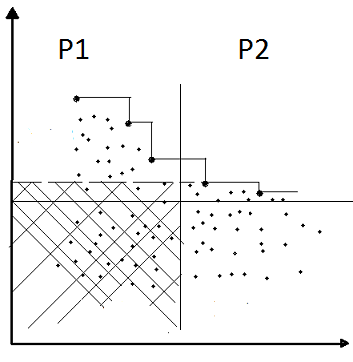
\includegraphics[width=60mm]{p2.png}
\caption{Figure for non-dominated pts}
\label{figp2}
\end{figure}

Proof by induction on size of set P.
\begin{itemize}
 \item If($\mid$P$\mid$=1), the point is non-dominated, hence the set P should be returned.
 \item If($\mid$P$\mid$=2), Remove dominanted point if exists, and return P.
 \item \textbf{Induction Hypothesis: } 
 As shown in figure, the points in $P_2$ have x-coordinate of any point is greater than x-coordinate of any point in $P_1$.\\
 See figure(\ref{figp2}).\\
 If p* is the point with maximum y-coordinate in $P_2$, any point in $P_1$ which has y-coordinate greater than that of p* can be dominated by the point
  p*.\\
 Thus, the group of points in $P_1$ that have y-coordinate less than that of p* are dominated, hence need to be removed.\\
 Hence, we need to remove this group of points from $P_1$ and solution of $P_1$ $ \cup$ solution of $P_2$ will be the answer.\\
 Thus, the algorithm is correct.
\end{itemize}
\newpage

\paragraph{Pseudo-Code.} \mbox{} \\
\begin{algorithm}

NonDominatedPts(set of points P)\{\\
\makebox[40pt]{}\textcolor{blue}{//Returns set of non dominated points from $P$.}\\
\Begin{
      \uIf{$\mid$P$\mid$==1} {return P\;}
      \uElseIf{$\mid$P$\mid$==2}{
	    let $p_1$ and $p_2$ be the two points in P\;
	    \uIf {$x_1 > x_2$ and $y_1 > y_2$}{ return \{$p_1$\};	\qquad	\textcolor{blue}{//$p_1$=($x_1$,$y_1$), and $p_2$=($x_2$,$y_2$)}}\\
	    \uElseIf{$x_1 < x_2$ and $y_1 < y_2$} {return \{$p_2$\}\;}   
	    \uElse{return P;}
      }
      \uElse{
	    p* $\gets$ x-median(P)\;
	    (L,R) $\gets$ split(P, p*)\;
	    L $\gets$ L sorted along y-axis\;
	    y $\gets$ max y-coordinate in points of R\;
	    L $\gets$ L - \{all points in L whose y-coordinate $\leq$ y\} \;
	    $P_1$ $\gets$ NonDominatedPts(L)\;
	    $P_2$ $\gets$ NonDominatedPts(R)\;
	    return ($P_1\cup P_2$) \;
      }
 }
\}
\caption{\textbf{$O(n logh)$} algorithm to find Non Dominated Points}
\end{algorithm}
\newpage

\subsection{\textbf{$O(i logi)$} algorithm to maintain non-dominated points in online fashion}

\paragraph{Introduction:} \makebox[2pt]{}\\\\
Data Structure used: Height Balanced Binary Search Tree (T).\\
Apart from value($i.e.$ x-coordinate), left, right, we will augment tree with another pointer \textbf{predecessor}
that stores the predecessor of the node in the tree $T$($i.e.$ the node which has x-coordinate just before this node).
\paragraph{Functions used:} 
\begin{enumerate}
 \item
 Insert($p_{new}$, T): It is used to insert $p_{new}$ in BST tree $T$ such that T remains height balanced.
 \item 
  FindSuccessor(T, $p_{new}$): Used to find the successor of the point before it is inserted into BST T.
  \item
 Delete(T, $p$): Delete point p from tree T.\\
\makebox[40pt]{}We will just need to follow the path where the point will be inserted, initialise successor to null, 
whenever we move right from a node, this cannot be the successor,
so ignore this node. Whenever we move to left of a node, this can be a possible successor, hence update successor. When we reach the
position where this new node will be inserted, the value of successor is returned. \\
\textbf{Time Complexity:} $\textbf{O(log i)}$.
\item
FindMax(): Keep traversing to the right, till right of the node is null, this node will be the maximum of the tree.
\end{enumerate}
\paragraph{Idea (What We are trying to do?)} \makebox[2pt]{}
\begin{itemize}
 \item We are placing the NonDominated(ND) points in a BST(height balanced) according to x-coordinate as key of BST.
 \item When a new point, $p_{new}$ is inserted in the graph, its y-coordinate is compared with its successor for being a ND point.
    \begin{itemize}
    \item If its y-coordinate is less than y-coordinate of its successor, then simply ignore the new point. 
    \item Else if its y-coordinate is greater than its successor, then it is a non-dominated point as well as the successor is non-dominated. Hence, 
    insert $p_{new}$.
    \end{itemize}
 \item Subsequently, if the point $p_{new}$ passes the comparison test with its successor $s$, after inserting $p_{new}$, all other ND-Points,
 existing above the successor of $p_{new}$ in the tree(with x-coordinate less than x-coordinate of $p_{new}$),
 need to be compared with $p_{new}$ to check if they still are non-dominanted.
 \item Those who fail the test are deleted from the tree.
 \item The test stops if we reach the top of the ND staircase or a ND Point successfully passes the comparison test with point P
 (note if a point is not deleted, then none of its predecessors need to be deleted anymore).
\end{itemize}

\paragraph{Time Complexity:} \textbf{$O(i logi)$}.\\
At each insertion of points into the graph, points will be either inserted or deleted from the tree which takes
$O(log k)$ time, where k$\leq$ i is the number of elements in the tree T.\\
Therefore overall time complexity for I steps of insertion is $O(i log i)$.

\newpage
\begin{algorithm}
\paragraph{Pseudo Code:}\makebox[2pt]{}\\
\makebox[2pt]{}\\AddNewPoint($p_{new}$, T)\{\\
\Begin{

  \eIf{T== \textcolor{red}{NULL} }{
 	Insert($p_{new}$,T)\;
 	$p_{new}\rightarrow$predecessor = \textcolor{red}{NULL}\;
  }{
       successor = FindSuccessor(T, $p_{new}$)\;
       \uIf{successor == \textcolor{red}{NULL}}{
	    $p_{new}\rightarrow$predecessor = FindMax()\;
       }
      \uElseIf{successor$\rightarrow$y $<$ $p_{new}\rightarrow$y}{
	Insert($p_{new}$, T)\;
 	temp1 = successor$\rightarrow$predecessor\;
 	successor$\rightarrow$predecessor = $p_{new}$\;
 	\While {temp1 $<>$ \textcolor{red}{NULL} and temp1$\rightarrow$ y $<$ $p_{new}\rightarrow$y}{
	  temp2 = temp1$\rightarrow$predecessor\;
 	  Delete(T, temp1)\;
 	  temp1 = temp2\;
 	}
 	P$\rightarrow$predecessor = temp1\;
      }
      \uElse{
	  \textcolor{blue}{//Ignore $p_{new}$.}\\
      }
    }\makebox[2pt]{}\\
}
\}
\caption{\textbf{$O(i logi)$} algorithm to maintain non dominated points}
\label{algo}
\end{algorithm}
\newpage
\paragraph{Proof of Correctness:} \makebox[2pt]{}\\
\begin{figure}[ht!]
\centering
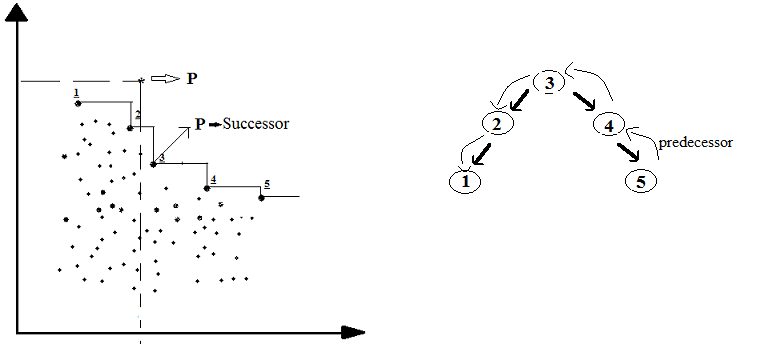
\includegraphics[width=100mm]{p11.png}
\caption{Case 1}
\label{fig1}
\end{figure}
\paragraph{Case 1:} \makebox[2pt]{}\\
In this case, P passes its comparison test with its successor (3) but 1 and 2 fail their comparison test
with P because P’s x and y coordinates are both high compared to them. Therefore points 1 and 2 will be deleted
from the tree T and point 3’s predecessor will be P.\\
\begin{figure}[ht!]
\centering
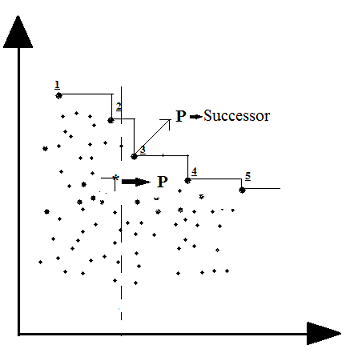
\includegraphics[width=50mm]{p12.png}
\caption{Case 2}
\label{fig2}
\end{figure}
\paragraph{Case 2:} \makebox[2pt]{}\\
In this case where P's y coordinate is less compared to its successor (3), it fails to become a ND Point
and therefore, the tree remains as it was before the insertion of P into the plane.

\newpage
\subsection{Non Dominated Points in a 3D plane}
\paragraph{Introduction:} \makebox[2pt]{}\\
In the case where the points are arranged  in a 3D space, the solution
for calculating all the non-dominant points will remain similar to algorithm \ref{algo} with few modifications.\\\\
Data Structure used: Height Balanced Binary Search Tree(T).
\paragraph{Functions used:}
\begin{enumerate}
 \item 
 FindSuccessor(T, $p_{new}$): Used to find the successor of the point before it is inserted into BST T.(Same as that in 1(c).)
\item
FindMax(): Keep traversing to the right, till right of the node is null, this node will be the maximum of the tree.
 \item
 Insert($p_{new}$,T): It is used to insert a node into tree T such that it remains balanced.
 \item
 Delete(T, $p$): Delete point p from tree T.
 \item
 All these functions take O(log n) time, where n is the size of tree T. 
\end{enumerate}
Note here only the left and right child pointer in the nodes of T need to be stored. Predecessor pointer
is not needed.
\paragraph{Idea(what we are trying to do:)}
\begin{itemize}
 \item 
We look at the 3D plane from a particular axis (z) i.e. the points are first sorted according to decreasing order of their z coordinates.
\item
The outermost ND Points are stored in tree T according to increasing order of their x coordinate and the remaining ND Points are stored in a separate array.
\item
As we move from the top of the z axis, the point P’s successor (in the tree T) is computed and its y coordinate is compared with P.
\item
Subsequently, if the point P passes the comparison test with its successor (temp), all other ND Points above temp are compared with P. If their y coordinate is less than P then they
are removed from the tree and inserted into an array (Points which are also Non Dominated) because their z coordinate is large compared to P.
\item
The test stops when we reach the top of the ND staircase or a ND Point above P has high Y coordinate compared to point P.
\end{itemize}

\paragraph{Time complexity:}
\begin{itemize}
 \item 
Sorting according to z coordinate takes $O(n log n)$ time.
\item
Inserting into array take $O(1)$ time.
\item
Deleting from tree takes $O(log n)$ time, if all nodes are deleted at the same time, it will take $O(n logn)$.
\end{itemize}

Hence the overall time complexity remains $O(n log n)$ for n points in the plane.

\begin{algorithm}
\paragraph{Pseudo Code:}\makebox[2pt]{}\\
\makebox[2pt]{}\\
BuildNonDominatedPtsTree($P$)\{\\
\Begin{
  Sort points according to decreasing order of z-coordinate.\\
  Array Points[]\;
  \eIf{T== \textcolor{red}{NULL} }{
 	Insert($p_{new}$,T)\;
 	$p_{new}\rightarrow$predecessor = \textcolor{red}{NULL}\;
  }{
       successor = FindSuccessor(T, $p_{new}$)\;
       \uIf{successor == \textcolor{red}{NULL}}{
	  Insert($p_{new}$,T)\;
	  $p_{new}\rightarrow$predecessor = FindMax()\;
       }
      \uElseIf{successor$\rightarrow$y $<$ $p_{new}\rightarrow$y}{
	Insert($p_{new}$, T)\;
 	temp1 = successor$\rightarrow$predecessor\;
 	successor$\rightarrow$predecessor = $p_{new}$\;
 	\While {temp1 $<>$ \textcolor{red}{NULL} and temp1$\rightarrow$ y $<$ $p_{new}\rightarrow$y}{
	  temp2 = temp1$\rightarrow$predecessor\;
	  Points.add(temp1)\;
 	  Delete(T, temp1)\;
 	  temp1 = temp2\;
 	}
 	P$\rightarrow$predecessor = temp1\;
      }
      \uElse{
	  \textcolor{blue}{//Ignore $p_{new}$.}\\
      }
    }\makebox[2pt]{}\\
    return $T$\;
}
\} \makebox[2pt]{}\\
ReportNonDominatedPoints(P)\{\\
\Begin{
    T = BuildNonDominatedPtsTree($P$)\;
    Output $T \cup Points[ ]$\;
}
\}\\
\caption{$\textbf{O(n log n)}$Finding Non Dominated Points in 3D plane.}
\end{algorithm}
\newpage
\paragraph{Proof of Correctness:} \makebox[2pt]{}\\
We have sorted the points in the decreasing order of z-coordinate and started seeing the points from the top of Z-axis.\\
\begin{itemize}
 \item 
 Base case: When the first point P is inserted, its successor in T(which is maintained according to increasing order of x- coordinate) is NULL, therefore, it is inserted T. 
The base case is obviously correct as this is the only point and hence has to be Non Dominated.
\item Induction Hypothesis: We assume that before we move upto I points, the tree T and array (Points)
contains the non-dominated points.
 \item Induction Step: We  need to show that this  algorithm works correctly for the $i^{th}$ point (P). Following cases are possible:
 \begin{itemize}
  \item 
  If the successor of point P in T is found out to be NULL, then it implies
that the x-coordinate of P is more than all the ND points stored  in T. Therefore,
P is inserted into T as no other point is dominating it.
Also, all the points above P in the staircase formation (Predecessor of P in T) with y-coordinates less than that of P are moved from T to be stored separately in the array (Points).
since their z-coordinates are higher than that of P they are also a set of Non-dominating points.
 \item If the successor  of ith point in T is found out not to be NULL, then following cases can occur:
 \begin{itemize}
  \item If the y-coordinate of successor is greater than that of P, then this point is clearly dominated by the successor because P’s x,y and z coordinates are smaller than that of its successor.
Hence point P is not inserted in the tree T.
 \item If the y-coordinate of successor is less than that of P, then no point in T dominates P and hence the point P is inserted in T and all the prede-
cessor of P in T with y-coordinates smaller than that of P is moved from T to array (Points)
to maintain the stair-case but stored separately as described in case1.
 \end{itemize}
 
 \end{itemize}
From the induction step, it is clear that we are correctly updating the tree T to contain the set of
ND points according to the most recently processed point.

 \end{itemize}
\newpage
\section{A computational problem of experimental physicist}

The total force on $i_{th}$ particle is given as:
\begin{center}
$F_j$ = $\Sigma_{i<j} \frac{Cq_i q_j}{(j-i)^2}$ - $\Sigma_{i>j} \frac{Cq_i q_j}{(j-i)^2}$
\end{center}
where the first $\Sigma$ denotes forces from the left, and the second $\Sigma$ denotes forces from the right.

This calculation of the terms takes $O(n)$ for each j. Thus making the time complexity of the program $O(n^2)$.\\
If we can calculate these summation faster, we can calculate the force efficiently.\\
Force on $q_2$:\\
$F_2$ = $\Sigma_{i<2} \frac{Cq_i q_2}{(2-i)^2}$ - $\Sigma_{i>2} \frac{Cq_i q_2}{(2-i)^2}$
= $\frac{Cq_1 q_2}{1^2}$ - $\frac{Cq_3 q_2}{1^2}$ - $\frac{Cq_4 q_2}{(4-2)^2}$ - \ldots\\\\
Using polynomials,
\begin{center}
$A(x)$ = $q_1$ + $q_2 x$ + $q_3 x^2$ + \ldots + $q_n x^{n-1}$\\
= $\Sigma_{i=1}^{n} q_i x^{i-1}$.\\\makebox[2pt]{} \\

$B(x)$ = $q_n$ + $q_{n-1} x$ + $q_{n-2} x^2$ + \ldots + $q_1 x^{n-1}$\\
= $\Sigma_{i=n}^{1} q_i x^{n-i}$.\\\makebox[2pt]{} \\

$C(x)$ = $(\frac{1}{1^2})$ + $(\frac{1}{2^2}) x$ + $(\frac{1}{3^2}) x^2$ + \ldots + $(\frac{1}{(n)^2}) x^{n-1}$\\
= $\Sigma_{i=1}^{n} (\frac{1}{i^2}) x^{i-1}$.\\\makebox[2pt]{} \\

$D(x)$ = $A(x) * C(x)$ \\\makebox[2pt]{}\\ = $\frac{q_1}{1^2}$ + $[(\frac{q_1}{2^2})+(\frac{q_2}{1^2})] x$ + 
			     $[(\frac{q_1}{3^2}) + (\frac{q_2}{2^2}) + (\frac{q_3}{1^2})] x^2$ + \ldots + $[(\frac{q_1}{n-1^2})+(\frac{q_2}{n-2^2})+$ \ldots $+(\frac{q_{n-1}}{n-1^2})] x^{n-2}$
			     +$ \frac{q_n}{n^2} x^{2n-2}$\\\makebox[2pt]{}\\

$E(x)$ = $B(x) * C(x)$ \\\makebox[2pt]{}\\ = $\frac{q_n}{1^2}$ + $[(\frac{q_n}{2^2})+(\frac{q_{n-1}}{1^2})] x$ + 
			     $[(\frac{q_n}{3^2}) + (\frac{q_{n-1}}{2^2}) + (\frac{q_{n-2}}{1^2})] x^2$ + \ldots + $[(\frac{q_n}{n-1^2})+(\frac{q_{n-1}}{n-2^2})+$ \ldots $+(\frac{q_{2}}{1^2})] x^{n-2}$
			     +$ \frac{q_1}{n^2} x^{2n-2}$\\\makebox[2pt]{}\\

\end{center}
\newpage

\paragraph{Observation:}

The coefficient of $x^0$ in $D(x)$ is the force from the left on $q_2$ divided by C*$q_2$, coefficient of $x^1$ is the force from the
left on $q_3$ divided by C*$q_3$, and hence from left on $q_{i}^{th}$ particle is coefficient of $x^{i-1}$(i is from 1 to n), divided by C*$q_i$.\\\\
And the coefficient of $x^0$ in $E(x)$ is the force on the $(n-1)^{th}$ particle from the right, divided by C*$q_{n-1}$, 
and the coefficient of $x^1$ is the force on the $(n-2)^{th}$ particle from the right divided by C*$q_{n-2}$, and so on. 
The $(n-2)^{th}$ term (coefficient of $x^{n-2}$) is the force on $q_1$ from the right divided by C*$q_{1}$. 
Hence $i^{th}$ term upto $(n-2)^{th}$ terms is the force from right on $q_{n-i}^{th}$ particle, divided by C*$q_{n-i}$.\\

\paragraph{Points to note:}
\begin{itemize}
 \item 
 This also covers the corner cases, $i.e.$ force from left on $1^{st}$ particle is coefficient of C*$q_1*$ coefficient of $x^{-1}$, $i.e.$ 0.
 \item
 Similarly, force on $q_n$ from right is coefficient of $x^{-1}$, $i.e.$ 0.
 \item
 We only need to consider coefficient of terms upto $x^{n-2}$. The terms coming later are not relevant to this algorithm. 
 Hence, we can discard them or rather not compute them.
 \item
 The Product function used in following pseudo code is the polynomial multiplication taught in class, that takes $O(n log n)$ time to multiply 
 two polynomials. We will assume this function returns the product polynomial in an array, with index $i$ from 0 to n-1(note we assumed i from 1 to n above).
\end{itemize}

\paragraph{Proof of correctness:} \makebox[2pt]{}\\\\
Looking at the general term of $D(x)$ and $E(x)$, force on particle $q_j$ as given by the algorithm will be:
\begin{center}
 C * $q_j$ * [($\Sigma_{i=1}^{j-1} (\frac{q_i}{(j-i)^2})$) - ($\Sigma_{i=j+1}^{n} (\frac{q_i}{(j-i)^2})$)].
\end{center}
which is equal to $F_j$ as given in the formula.\\
Hence, the algorithm is correct.

\newpage

\paragraph{Pseudo Code}\mbox{} \\
\begin{algorithm}
Output$F_j$(array $q_i$[ ])\{\\
\Begin{
      $A(x)$ $\gets$ $q_1$ + $q_2 x$ + $q_3 x^2$ + \ldots + $q_n x^{n-1}$ \;
      $B(x)$ $\gets$ $q_n$ + $q_{n-1} x$ + $q_{n-2} x^2$ + \ldots + $q_1 x^{n-1}$ \;
      $C(x)$ $\gets$ ($\frac{1}{1^2}$) + ($\frac{1}{2^2}) x^2$ + ($\frac{1}{3^2}) x^3$ + \ldots + ($\frac{1}{n^2}) x^{n-1}$\;
      \makebox[40pt]{}\textcolor{blue}{//The algorithm of product returns array D where element \makebox[40pt]{}//D[i] is the $i^{th}$ coefficient, i goes from 0 to n-1.}\\
      $D(x)$ $\gets$ Product($A(x), C(x)$);\makebox[40pt]{}\textcolor{red}{//O($c_1$n logn)}\\
      $E(x)$ $\gets$ Product($B(x), C(x)$);\makebox[40pt]{}\textcolor{red}{//O($c_2$n logn)}\\
      \For{$i \leftarrow 1$ \KwTo $n$}{
	Output C * $q_i$ * (Coefficient(D, i-2) - Coefficient(E, n-i-1))\;	\makebox[40pt]{}\textcolor{blue}{//C is the coulomb's constant.\\\makebox[40pt]{}//
	The Coefficient(P,i) function returns the coefficient \\\makebox[40pt]{}//of $x^i$ in polynomial P.}
      }\textcolor{red}{//($c_3$n) for loop}
}
\}
\\\makebox[2pt]{}\\
Coefficient(polynomial P, exponent i)\{\makebox[40pt]{}\textcolor{blue}{//O(1) time.}\\\makebox[40pt]{}\textcolor{blue}{//The polynomial is kept as an array.}\\
\Begin{
    \eIf{$i<0$}{
	return 0\;
    }{
	return P[i]\;
    }
}
\}
\caption{Pseudo Code for finding forces on particles}
\end{algorithm}
\\
\paragraph{Time Complexity:} \makebox[2pt]{}\\
The text in red shows the time taken by the algorithm is (($c_1+c_2$) n logn + $c_3$n), hence time complexity of the algorithm is \textbf{$O(n logn)$}.

\end{document}